\section{D.Irga B. Naufal Fakhri (1174066)}
\subsection{Teori}

\subsubsection{Apa Itu Random Forest}

\hfill\break
Random Forest adalah sebuah algoritma yang digunakan terhadap klasifikasi data dalam jumlah yang besar. Klasifikasi pada random forest dilakukan dengan penggabungan dicision tree dengan melakuakn training terhadap sempel data yang dimiliki. Semakin banyak dicision tree maka data yang di dapat akan
semakin akurat.
\begin{figure}[H]
\centerline{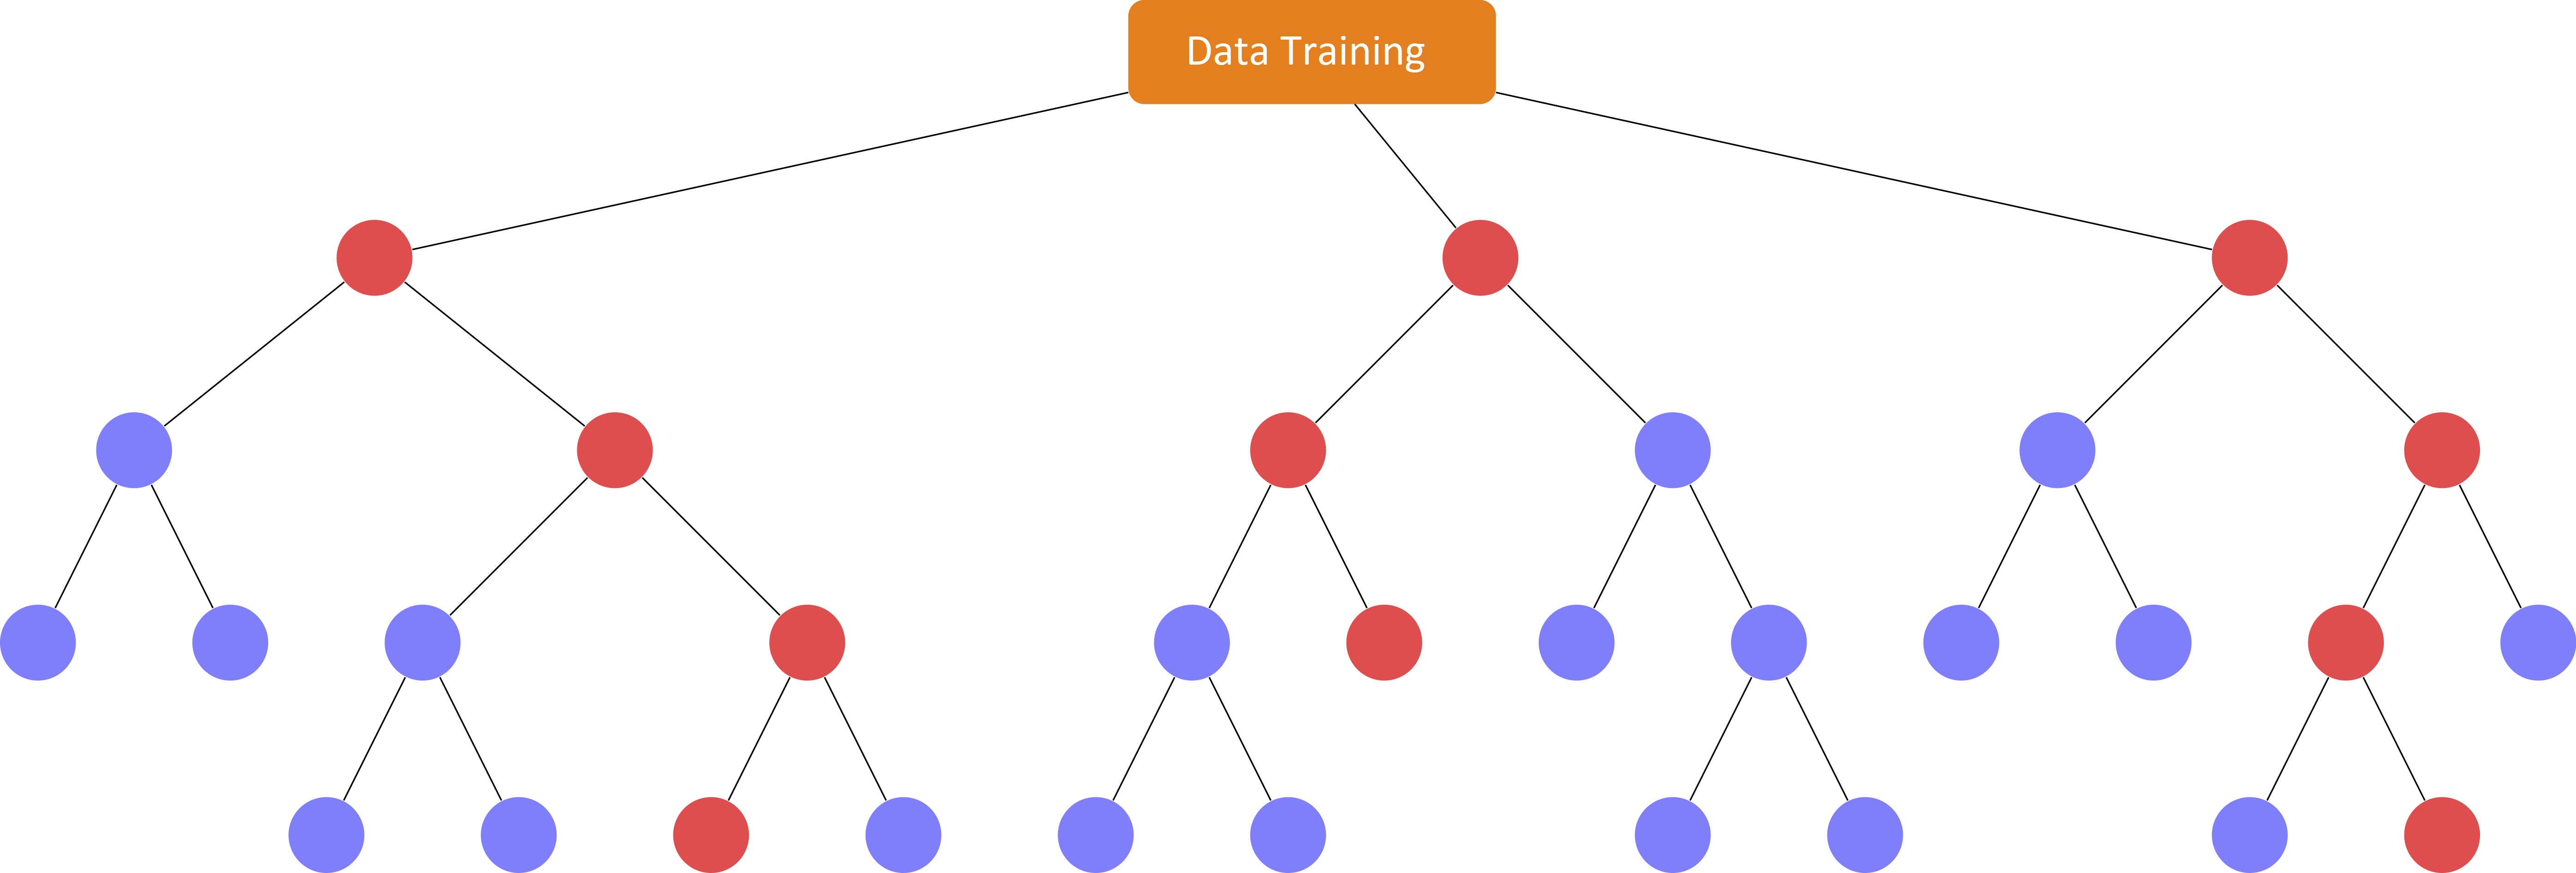
\includegraphics[width=10cm]{figures/1174066/3/1.jpg}}
\caption{Random Forest}
\label{labelgambar}
\end{figure}

\subsubsection{cara membaca dataset kasus dan artikan makna setiap file dan isi field masing-masing file.}

\hfill\break
\begin{itemize}
\item Pertama download dataset terlebih dahulu lalu buka dengan menggunakan software spyder guna melihat isi dari dataset tersebut.

\item Data tersebut memiliki extensi file bernama .txt dan didalamnya terdapat class dari field.

\item Misalnya saja pada data jenis burung memiliki file index dan angka, dimana index berisi angka yang memiliki makna berupa jenis burung.

\item bahkan nama burung sedangkan field memiliki isi nilai berupa 0 dan 1 yang dimana sifatnya boolean atau Ya dan Tidak.

\item Hal ini dikarenakan komputer hanya dapat membaca bilangan biner maka dari itu field yang di isikan berupa angka.

\item Artinya angka 0 berarti tidak dan angka 1 berarti Ya.
\end{itemize}

\subsubsection{Cross Validation}

\hfill\break
Cross Validation adalah sebuah teknik validasi model yang berfungsi untuk melakukan penilaian bagaimana hasil analisis statistik akan digeneralisasi ke data yang lebih independen. Cross validation digunakan dengan tujuan prediksi, dan bila kita ingin memperkirakan seberapa akurat model model prediksi yang dilakukan dalam sebuah praktek. Tujuan dari cross validation yaitu untuk mendefinisikan dataset guna menguju dalam fase pelatihan untuk membatasi masalah seperti overfitting dan underfitting serta mendapatkan wawasan tentang bagaimana model akan digeneralisasikan ke set data independen.

\subsubsection{Arti score 44 \% pada random forest, 27\% pada decission tree dan 29 \% dari SVM.}

\hfill\break
Dimana Score 44 \% didapatkan dari hasil pengelohan dataset jenis burung. Dimana akan dilakukan proses pembagian data testing dan data training lalu diproses dan menghasilkan score sebanyak 44 \% dimana menjelaskan bahwa score tersebut digunakan sebagai pembanding dalam tingkat keakuratannya. Pada dicision tree akan memperoleh data lebih kecil yaitu sebanyak 27 \% hal ini dikarenakan data yang diolah menggunakan dicision tree dibagi menjadi beberapa tree dan lalu disimpulkan untuk mendapatkan data yang akurat. Pada SVM akan memperoleh score sebanyak 29 \% hal ini dikarenakan data yang dimiliki masih bernilai netral sehingga tingkat keakuratannya masih belum jelas.

\subsubsection{Cara membaca confusion matriks dan contohnya memakai gambar atau ilustrasi sendiri.}

\hfill\break
Perthitungan Confusion Matriks dapat dilakukan dengan cara dibawah ini.
\begin{itemize}
\item
Import librari Pandas, Matplotlib, dan Numpy.
\item
Buat variabel y actu yang berisikan data aktual.
\item
Buat variabel y pred berisikan data yang akan dijadikan sebagai prediksi.
\item
Buat variabel df confusion yang berisikan crosstab untuk membangun tabel tabulasi silang yang dapat menunjukkan frekuensi kemunculan kelompok data tertentu.
\item
Pada variabel df confusion definisikan lagi nama baris yaitu Actual dan kolomnya Predicted
\item
Kemudian definisikan suatu fungsi yang diberi nama plot confusion matrix yang berisikan pendefinisian confusion matrix dan juga akan di plotting.
\lstinputlisting{src/1174066/3/conmatriks.py}
\end{itemize}
\begin{figure}[H]
\centerline{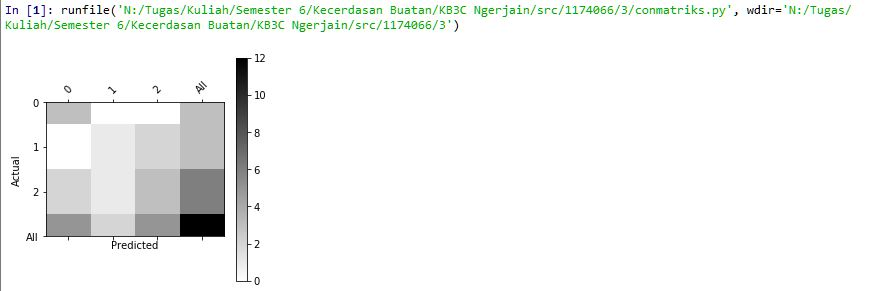
\includegraphics[width=10cm]{figures/1174066/3/2.jpg}}
\caption{Confusion Matriks}
\label{labelgambar}
\end{figure}

\subsubsection{Apa itu voting pada random forest}

\hfill\break
Voting yaitu suara untuk setiap target yang diprediksi pada saat melakukan Random Forest dilakukan. Pertimbangkan target prediksi dengan voting tertinggi sebagai prediksi akhir dari algoritma random forest.

Untuk menggunakan Voting pada Random Forest dapat dilihat code ini:
\lstinputlisting{src/1174066/3/voteforest.py}
\begin{figure}[H]
\centerline{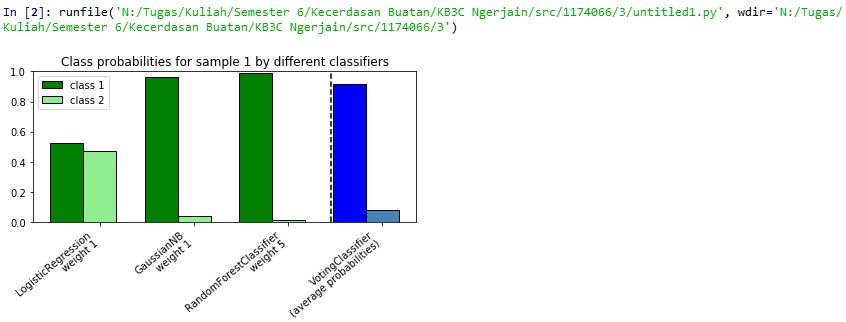
\includegraphics[width=10cm]{figures/1174066/3/3.jpg}}
\caption{Voting Random Matriks}
\label{labelgambar}
\end{figure}


\subsection{Praktek}
\subsubsection{Nomor 1}
\hfill\break
\lstinputlisting[firstline=8, lastline=13]{src/1174066/3/1174066.py}
\begin{figure}[H]
\centerline{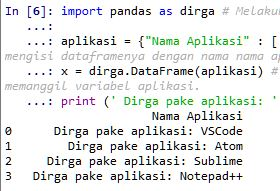
\includegraphics[width=10cm]{figures/1174066/3/4.jpg}}
\caption{Membuat Aplikasi pakai pandas}
\label{labelgambar}
\end{figure}

\subsubsection{Nomor 2}
\hfill\break
\lstinputlisting[firstline=16, lastline=21]{src/1174066/3/1174066.py}
\begin{figure}[H]
\centerline{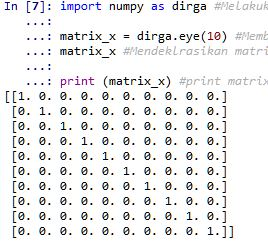
\includegraphics[width=10cm]{figures/1174066/3/5.jpg}}
\caption{Membuat Aplikasi pakai numpy}
\label{labelgambar}
\end{figure}

\subsubsection{Nomor 3}
\hfill\break
\lstinputlisting[firstline=24, lastline=28]{src/1174066/3/1174066.py}
\begin{figure}[H]
\centerline{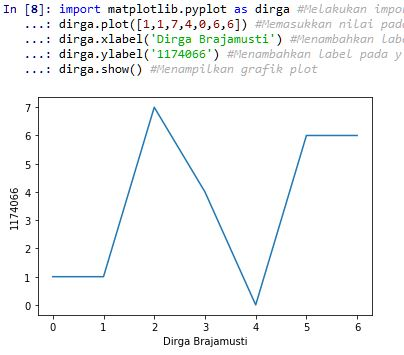
\includegraphics[width=10cm]{figures/1174066/3/6.jpg}}
\caption{Membuat Aplikasi pakai matplotlib}
\label{labelgambar}
\end{figure}

\subsubsection{Nomor 4}
\hfill\break

\begin{itemize}
\item Source Code pertama pada random forest berfungsi untuk membaca dataset yang memiliki format text file dengan mendefinisikan variabel yang bernama imgatt. Variabel tersebut berisi value untuk membaca data.
\lstinputlisting[firstline=34, lastline=38]{src/1174066/3/1174066.py}
\begin{figure}[H]
\centerline{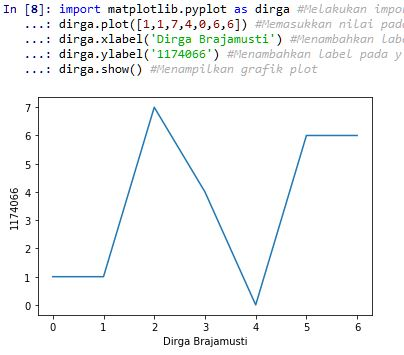
\includegraphics[width=10cm]{figures/1174066/3/6.jpg}}
\caption{Hasil 4 Bagian 1}
\label{labelgambar}
\end{figure}

\item Pada source code berikutnya akan mengembalikan baris teratas dari DataFrame variabel imgatt.
\lstinputlisting[firstline=42, lastline=43]{src/1174066/3/1174066.py}
\begin{figure}[H]
\centerline{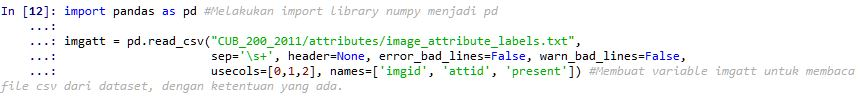
\includegraphics[width=10cm]{figures/1174066/3/7.jpg}}
\caption{Hasil 4 Bagian 2}
\label{labelgambar}
\end{figure}

\item Pada output berikutnya akan menampilkan jumlah kolom dan baris dari DataFrame variable imgatt.
\lstinputlisting[firstline=42, lastline=43]{src/1174066/3/1174066.py}
\begin{figure}[H]
\centerline{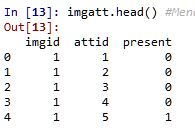
\includegraphics[width=10cm]{figures/1174066/3/8.jpg}}
\caption{Hasil 4 Bagian 3}
\label{labelgambar}
\end{figure}

\item Variabel imgatt2 telah menggunakan fungsi yang bernama pivot agar mengubah kolom jadi baris dan sebaliknya dari DataFrame imgatt sebelumnya.
\lstinputlisting[firstline=48, lastline=48]{src/1174066/3/1174066.py}
\begin{figure}[H]
\centerline{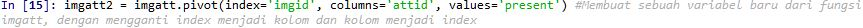
\includegraphics[width=10cm]{figures/1174066/3/10.jpg}}
\caption{Hasil 4 Bagian 4}
\label{labelgambar}
\end{figure}

\item Variabel imgatt2 head berfungsi untuk mengembalikan value teratas pada DataFrame imgatt2.
\lstinputlisting[firstline=51, lastline=51]{src/1174066/3/1174066.py}
\begin{figure}[H]
\centerline{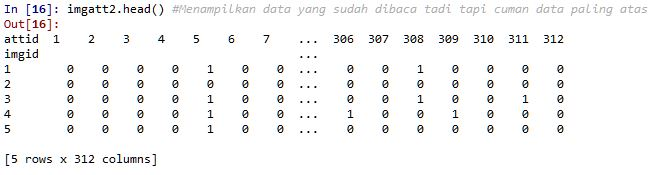
\includegraphics[width=10cm]{figures/1174066/3/11.jpg}}
\caption{Hasil 4 Bagian 5}
\label{labelgambar}
\end{figure}

\item Menghasilkan jumlah kolom dan baris pada DataFrame imgatt2.
\lstinputlisting[firstline=54, lastline=54]{src/1174066/3/1174066.py}
\begin{figure}[H]
\centerline{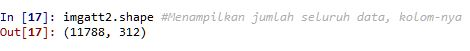
\includegraphics[width=10cm]{figures/1174066/3/12.jpg}}
\caption{Hasil 4 Bagian 6}
\label{labelgambar}
\end{figure}

\item Menunjukkan dalam melakukan pivot yang mana imgid menjadi sebuah index yang unik.
\lstinputlisting[firstline=62, lastline=65]{src/1174066/3/1174066.py}
\begin{figure}[H]
\centerline{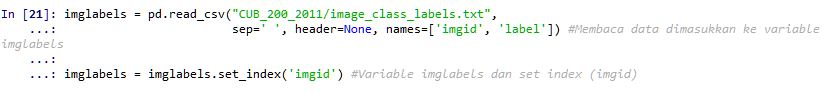
\includegraphics[width=10cm]{figures/1174066/3/13.jpg}}
\caption{Hasil 4 Bagian 7}
\label{labelgambar}
\end{figure}

\item Akan melakukan load jawabannya yang berisi apakah burung tersebut termasuk spesies yang mana. Kolom tersebut yaitu imgid dan label.
\lstinputlisting[firstline=68, lastline=68]{src/1174066/3/1174066.py}
\begin{figure}[H]
\centerline{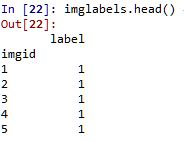
\includegraphics[width=10cm]{figures/1174066/3/14.jpg}}
\caption{Hasil 4 Bagian 8}
\label{labelgambar}
\end{figure}

\item Menunjukkan bahwa jumlah baris sebanyak 11788 dan kolom 1 yang dimana kolom tersebut adalah jenis spesies pada burung.
\lstinputlisting[firstline=71, lastline=71]{src/1174066/3/1174066.py}
\begin{figure}[H]
\centerline{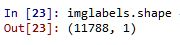
\includegraphics[width=10cm]{figures/1174066/3/15.jpg}}
\caption{Hasil 4 Bagian 9}
\label{labelgambar}
\end{figure}

\item Melakukan join antara imgatt2 dengan imglabels dikarenakan memiliki isi yang sama sehingga akan mendapatkan sebuah data ciri-ciri dan data jawaban sehingga bisa dikategorikan sebagai supervised learning.
\lstinputlisting[firstline=74, lastline=75]{src/1174066/3/1174066.py}
\begin{figure}[H]
\centerline{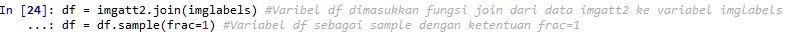
\includegraphics[width=10cm]{figures/1174066/3/16.jpg}}
\caption{Hasil 4 Bagian 10}
\label{labelgambar}
\end{figure}

\item Melakukan drop pada label yang ada didepan dan akan menggunakan label yang baru di joinkan.
\lstinputlisting[firstline=78, lastline=79]{src/1174066/3/1174066.py}
\begin{figure}[H]
\centerline{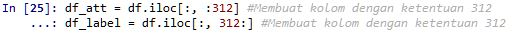
\includegraphics[width=10cm]{figures/1174066/3/17.jpg}}
\caption{Hasil 4 Bagian 11}
\label{labelgambar}
\end{figure}

\item Mengecek isi 5 data teratas pada df\_att.
\lstinputlisting[firstline=82, lastline=82]{src/1174066/3/1174066.py}
\begin{figure}[H]
\centerline{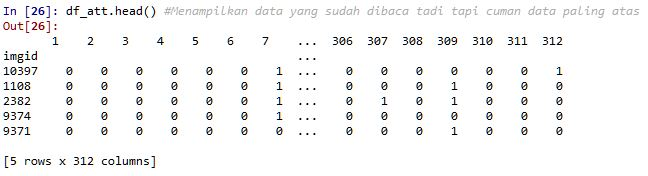
\includegraphics[width=10cm]{figures/1174066/3/18.jpg}}
\caption{Hasil 4 Bagian 12}
\label{labelgambar}
\end{figure}

\item Mengecek isi data teratas dari df\_label.
\lstinputlisting[firstline=85, lastline=85]{src/1174066/3/1174066.py}
\begin{figure}[H]
\centerline{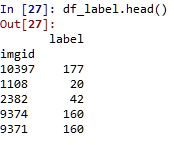
\includegraphics[width=10cm]{figures/1174066/3/19.jpg}}
\caption{Hasil 4 Bagian 13}
\label{labelgambar}
\end{figure}

\item Membagi 8000 row pertama menjadi data training dan sisanya adalah data testing.
\lstinputlisting[firstline=88, lastline=94]{src/1174066/3/1174066.py}
\begin{figure}[H]
\centerline{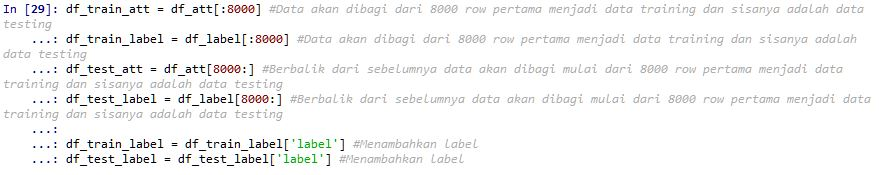
\includegraphics[width=10cm]{figures/1174066/3/20.jpg}}
\caption{Hasil 4 Bagian 14}
\label{labelgambar}
\end{figure}

\item Pemanggilan class RandomForestClassifier. Dimana artinya menunjukkan banyak kolom pada setiap tree adalah 50.
\lstinputlisting[firstline=97, lastline=98]{src/1174066/3/1174066.py}
\begin{figure}[H]
\centerline{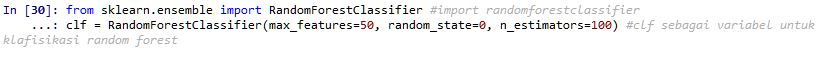
\includegraphics[width=10cm]{figures/1174066/3/21.jpg}}
\caption{Hasil 4 Bagian 15}
\label{labelgambar}
\end{figure}

\item Menunjukkan hasil prediksi dari Random Forest.
\lstinputlisting[firstline=101, lastline=101]{src/1174066/3/1174066.py}
\begin{figure}[H]
\centerline{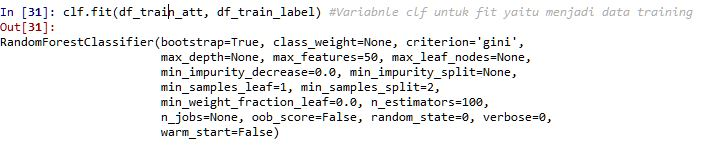
\includegraphics[width=10cm]{figures/1174066/3/22.jpg}}
\caption{Hasil 4 Bagian 16}
\label{labelgambar}
\end{figure}

\item Menampilkan besaran akurasi dari prediksi pada Random Forest yang merupakan score perolehan klarifikasi.
\lstinputlisting[firstline=104, lastline=104]{src/1174066/3/1174066.py}
\begin{figure}[H]
\centerline{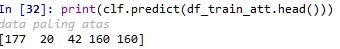
\includegraphics[width=10cm]{figures/1174066/3/23.jpg}}
\caption{Hasil 4 Bagian 17}
\label{labelgambar}
\end{figure}

\item Menampilkan besaran akurasi dari prediksi pada Random Forest yang merupakan score perolehan klarifikasi.
\lstinputlisting[firstline=107, lastline=107]{src/1174066/3/1174066.py}
\begin{figure}[H]
\centerline{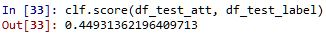
\includegraphics[width=10cm]{figures/1174066/3/24.jpg}}
\caption{Hasil 4 Bagian 18}
\label{labelgambar}
\end{figure}
\end{itemize}

\subsubsection{Nomor 5}
\hfill\break
\lstinputlisting[firstline=112, lastline=114]{src/1174066/3/1174066.py}
\begin{figure}[H]
\centerline{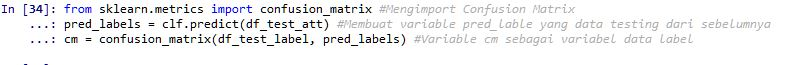
\includegraphics[width=10cm]{figures/1174066/3/25.jpg}}
\caption{Hasil 5 Bagian 1}
\label{labelgambar}
\end{figure}

\lstinputlisting[firstline=117, lastline=117]{src/1174066/3/1174066.py}
\begin{figure}[H]
\centerline{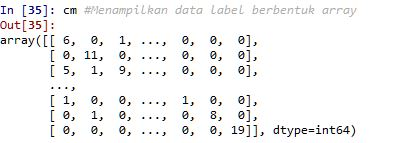
\includegraphics[width=10cm]{figures/1174066/3/26.jpg}}
\caption{Hasil 5 Bagian 2}
\label{labelgambar}
\end{figure}

\lstinputlisting[firstline=120, lastline=147]{src/1174066/3/1174066.py}
\begin{figure}[H]
\centerline{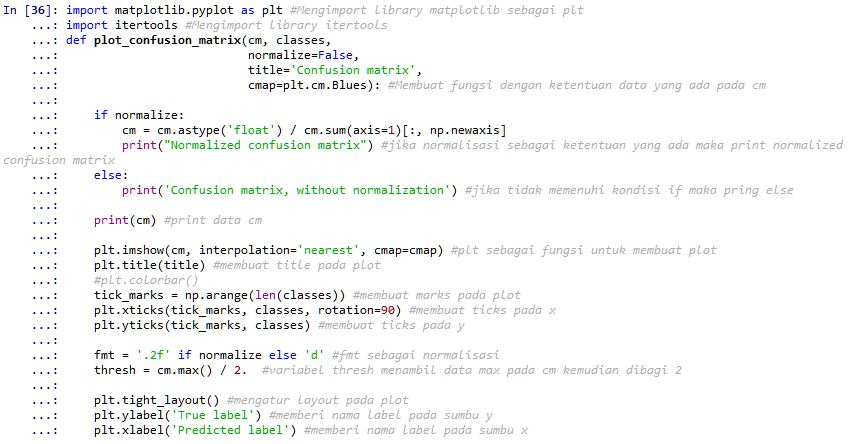
\includegraphics[width=10cm]{figures/1174066/3/27.jpg}}
\caption{Hasil 5 Bagian 3}
\label{labelgambar}
\end{figure}

\lstinputlisting[firstline=151, lastline=154]{src/1174066/3/1174066.py}
\begin{figure}[H]
\centerline{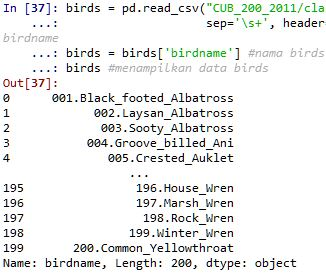
\includegraphics[width=10cm]{figures/1174066/3/28.jpg}}
\caption{Hasil 5 Bagian 4}
\label{labelgambar}
\end{figure}

\lstinputlisting[firstline=158, lastline=163]{src/1174066/3/1174066.py}
\begin{figure}[H]
\centerline{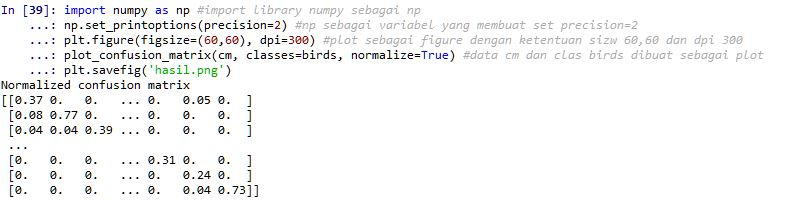
\includegraphics[width=10cm]{figures/1174066/3/29.jpg}}
\caption{Hasil 5 Bagian 5}
\label{labelgambar}
\end{figure}

\begin{figure}[H]
\centerline{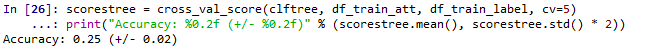
\includegraphics[width=10cm]{figures/1174066/3/30.png}}
\caption{Plot Hasil 5 Bagian 5}
\label{labelgambar}
\end{figure}

\subsubsection{Nomor 6}
\hfill\break
\lstinputlisting[firstline=168, lastline=171]{src/1174066/3/1174066.py}
\begin{figure}[H]
\centerline{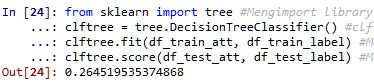
\includegraphics[width=10cm]{figures/1174066/3/31.jpg}}
\caption{Hasil 6 Bagian 1}
\label{labelgambar}
\end{figure}

\lstinputlisting[firstline=174, lastline=177]{src/1174066/3/1174066.py}
\begin{figure}[H]
\centerline{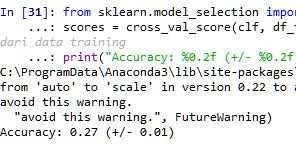
\includegraphics[width=10cm]{figures/1174066/3/32.jpg}}
\caption{Hasil 6 Bagian 2}
\label{labelgambar}
\end{figure}

\subsubsection{Nomor 7}
\hfill\break
\lstinputlisting[firstline=180, lastline=182]{src/1174066/3/1174066.py}
\begin{figure}[H]
\centerline{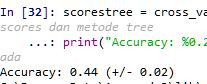
\includegraphics[width=10cm]{figures/1174066/3/33.jpg}}
\caption{Hasil 7 Bagian 1}
\label{labelgambar}
\end{figure}

\lstinputlisting[firstline=185, lastline=186]{src/1174066/3/1174066.py}
\begin{figure}[H]
\centerline{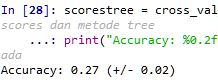
\includegraphics[width=10cm]{figures/1174066/3/34.jpg}}
\caption{Hasil 7 Bagian 2}
\label{labelgambar}
\end{figure}

\lstinputlisting[firstline=189, lastline=190]{src/1174066/3/1174066.py}
\begin{figure}[H]
\centerline{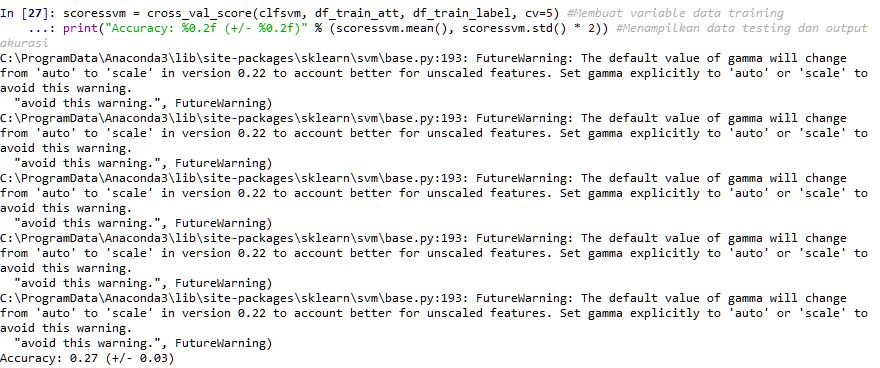
\includegraphics[width=10cm]{figures/1174066/3/35.jpg}}
\caption{Hasil 7 Bagian 3}
\label{labelgambar}
\end{figure}

\subsubsection{Nomor 8}
\hfill\break
\lstinputlisting[firstline=193, lastline=208]{src/1174066/3/1174066.py}
\begin{figure}[H]
\centerline{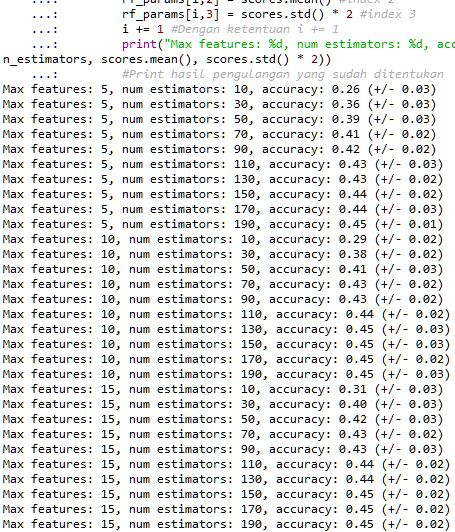
\includegraphics[width=10cm]{figures/1174066/3/36.jpg}}
\caption{Hasil 8 Bagian 1}
\label{labelgambar}
\end{figure}
\begin{figure}[H]
\centerline{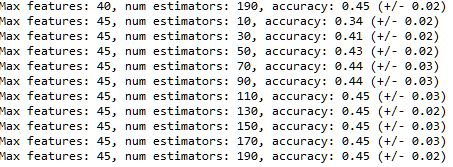
\includegraphics[width=10cm]{figures/1174066/3/37.jpg}}
\caption{Hasil 8 Bagian 1 Akhir kode}
\label{labelgambar}
\end{figure}

\lstinputlisting[firstline=210, lastline=224]{src/1174066/3/1174066.py}
\begin{figure}[H]
\centerline{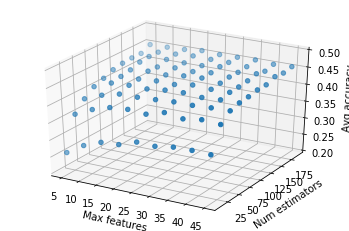
\includegraphics[width=10cm]{figures/1174066/3/38.png}}
\caption{Hasil 8 Bagian 2}
\label{labelgambar}
\end{figure}



\subsection{Penanganan Error}
\begin{enumerate}
	\item ScreenShoot Error
	\begin{figure}[H]
		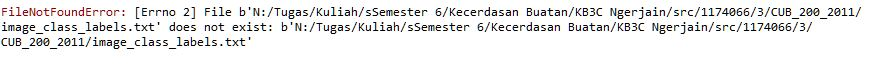
\includegraphics[width=4cm]{figures/1174066/3/error1.jpg}
		\centering
		\caption{FileNotFoundError}
	\end{figure}
	\item Tuliskan Kode Error dan Jenis Error
	\begin{itemize}
		\item FileNotFoundError
	\end{itemize}
	\item Cara Penangan Error
	\begin{itemize}
		\item FileNotFoundError
		\hfill\break
		Error terdapat pada kesalahan saat baca file csv, yang tidak terbaca. Dikarenakan letak file yang dibaca tidak para direktori yang sama. Seharusnya letakkan file di direktori yang sama. 
	\end{itemize}
\end{enumerate}


\subsection{Bukti Tidak Plagiat}
\hfill\\
\begin{figure}[H]
\centerline{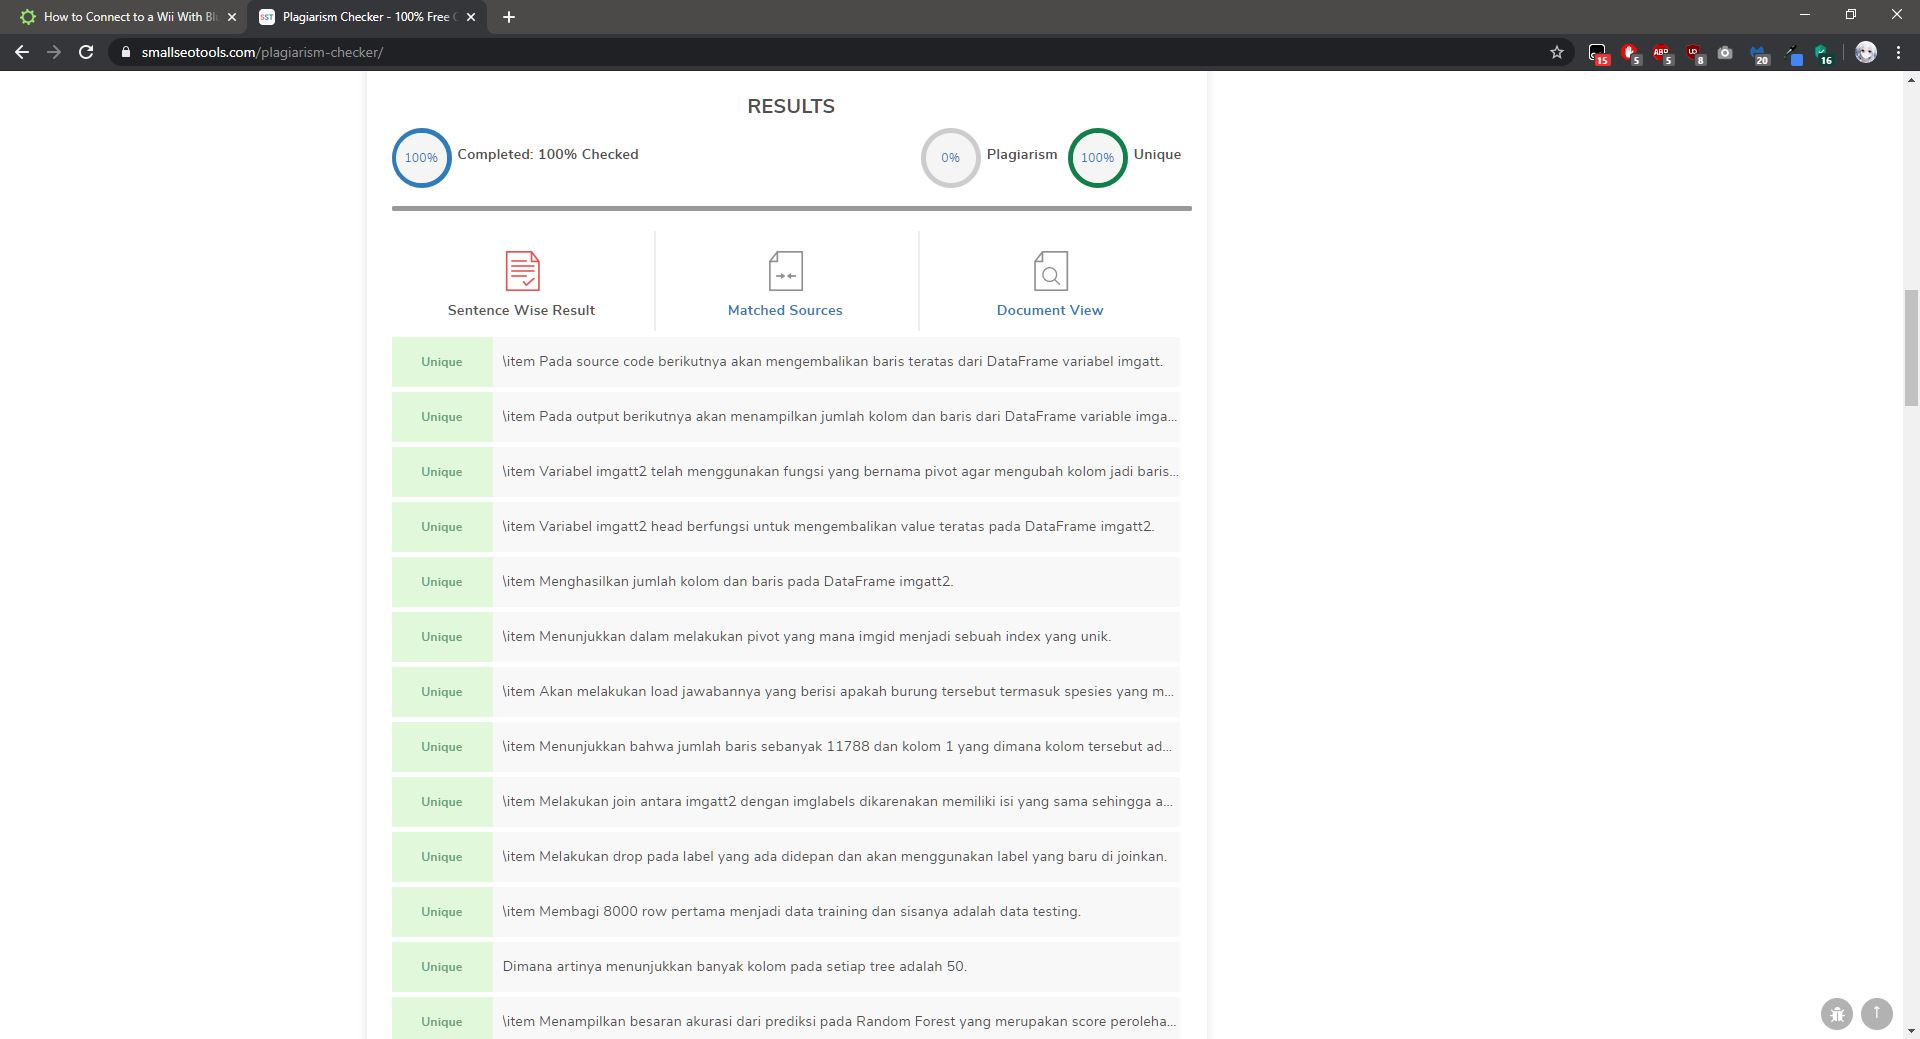
\includegraphics[width=10cm]{figures/1174066/3/plagiat.jpg}}
\caption{Bukti Tidak Plagiat}
\label{labelgambar}
\end{figure}

\subsection{Link Youtube:}
https://youtu.be/69BWGlcf\_CQ